\chapter{การแพร่กระจายของจุลินทรีย์ในสิ่งแวดล้อมและอากาศ}
\label{chap:ch02}

\section*{แผนบริหารการสอนประจำบทที่ 2}
\addcontentsline{toc}{section}{แผนบริหารการสอนประจำบทที่ 2}

\noindent\textbf{. หัวข้อเนื้อหาประจำบท}

\begin{enumerate}
    \item 2.1 แหล่งที่อยู่อาศัยและการกระจายตัวของจุลินทรีย์ในธรรมชาติ (Ubiquity of Microorganisms)
    \item 2.2 จุลินทรีย์ในอากาศ ดิน แหล่งน้ำธรรมชาติ และฝุ่นละออง
    \item 2.3 จุลินทรีย์ประจำถิ่นบนร่างกายมนุษย์ (Normal Flora of the Human Skin)
    \item 2.4 เทคนิคการเก็บตัวอย่างจากสิ่งแวดล้อมด้วยวิธีเปิดจานผึ่งอากาศและวิธี Swab
    \item 2.5 การนับและสังเกตลักษณะสัณฐานวิทยาของโคโลนี (Colony Morphology)
\end{enumerate}

\noindent\textbf{. วัตถุประสงค์เชิงพฤติกรรม}

\begin{enumerate}
    \item เมื่อนักศึกษาได้เรียนรู้และปฏิบัติการทดลองประจำบทนี้แล้ว จะต้องมีความรู้ความสามารถดังต่อไปนี้:
    \item อธิบายความหลากหลายและแหล่งแพร่กระจายของจุลินทรีย์ในสิ่งแวดล้อมประเภทต่างๆ ได้
    \item เก็บตัวอย่างจุลินทรีย์จากอากาศ ดิน น้ำ และผิวหนังด้วยวิธีปลอดเชื้อได้อย่างถูกต้อง
    \item ตรวจนับและจำแนกลักษณะโคโลนีของแบคทีเรียและเชื้อราบนจานอาหารเลี้ยงเชื้อได้
    \item เห็นคุณค่าของความสะอาดและสุขอนามัยส่วนบุคคลในการป้องกันการแพร่กระจายเชื้อ
\end{enumerate}

\noindent\textbf{. กิจกรรมการเรียนการสอน}

\begin{enumerate}
    \item การบรรยายสรุปก่อนปฏิบัติการ (30 นาที): อธิบายหลักการวิทยาศาสตร์ ความปลอดภัยทางชีวภาพ และข้อควรระวังสำคัญ
    \item การสาธิตเชิงประจักษ์ (15 นาที): สาธิตเทคนิคการปฏิบัติงาน การใช้เครื่องมือ และข้อผิดพลาดที่มักพบ
    \item การลงมือปฏิบัติการทดลองจริง (90 นาที): นักศึกษาลงมือปฏิบัติการทดลองเป็นรายบุคคลหรือกลุ่มย่อยตามขั้นตอนที่กำหนด
    \item การฝึกฝนผ่านระบบเสมือนจริง (20 นาที): ทดลองซ้ำและทดสอบปฏิกิริยาผ่านระบบจำลองบน RBRU LMS
    \item การอภิปรายและสรุปผลการทดลอง (25 นาที): วิเคราะห์ผลการสังเกต ตอบคำถามท้ายบท และสรุปองค์ความรู้ร่วมกัน
\end{enumerate}

\noindent\textbf{. สื่อและอุปกรณ์การเรียนการสอน}

\begin{enumerate}
    \item เอกสารคำสอนและคู่มือปฏิบัติการ: e-Book และคู่มือปฏิบัติการฉบับเต็ม ประจำบทที่ 2
    \item ระบบห้องปฏิบัติการเสมือนจริง: ระบบจำลองการทดลองเสมือนจริง 3 มิติ ประจำบทที่ 2 บนระบบ Moodle
    \item อุปกรณ์และเครื่องแก้วในห้องปฏิบัติการ: ตะเกียงแอลกอฮอล์, ห่วงเขี่ยเชื้อ, กล้องจุลทรรศน์, จานเพาะเชื้อ, หลอดทดลอง และตู้บ่มเชื้อ
    \item สารเคมีและสีย้อมชีวภาพ: สารเคมีมาตรฐานวิเคราะห์และสีย้อมประจำบทเรียน
\end{enumerate}

\noindent\textbf{. การวัดและประเมินผล}

\begin{table}[H]
\centering\small
\begin{tabularx}{\textwidth}{p{0.5\textwidth} p{0.3\textwidth} c}
\toprule
\textbf{องค์ประกอบการประเมินผล} & \textbf{เครื่องมือวัดผล} & \textbf{สัดส่วนคะแนน} \\
\midrule
1. ทักษะการปฏิบัติงานและความปลอดภัย & แบบสังเกตทักษะการทดลองและเทคนิคปลอดเชื้อ & 40\% \\
2. รายงานผลการทดลอง & การตรวจตารางบันทึกผล ภาพวาดสัณฐานวิทยา และการวิเคราะห์ผล & 30\% \\
3. แบบฝึกหัดทบทวนท้ายบท & คำถามทบทวนเชิงวิเคราะห์และข้อสอบท้ายบท & 20\% \\
4. จิตพิสัยและการตรงต่อเวลา & การเช็คชื่อ การแต่งกายตามระเบียบ และการทำความสะอาดโต๊ะแล็บ & 10\% \\
รวมทั้งสิ้น &  & 100\% \\
\bottomrule
\end{tabularx}
\end{table}

\newpage

% ==========================================================
% เนื้อหาบทเรียนประจำบทที่ 2
% ==========================================================

\section{การกระจายตัวของจุลินทรีย์ในชีวมณฑล}
\index{การกระจายตัวของจุลินทรีย์ในชีวมณฑล}

การศึกษาและทำความเข้าใจเกี่ยวกับการกระจายตัวของจุลินทรีย์ในชีวมณฑล (Ubiquity of Microorganisms) มีความสำคัญอย่างยิ่งในงานจุลชีววิทยาและสิ่งแวดล้อม โดยมีรายละเอียดสาระสำคัญดังนี้

จุลินทรีย์จัดเป็นสิ่งมีชีวิตที่พบได้ทั่วไปในทุกระบบนิเวศ (Ubiquitous organisms) ไม่ว่าจะเป็นในอากาศ แหล่งน้ำจืด น้ำทะเล ดิน อนุภาคฝุ่นละออง หรือบนพื้นผิวของสิ่งไม่มีชีวิต ตลอดจนร่างกายของสิ่งมีชีวิต

ในบรรยากาศ จุลินทรีย์มักแขวนลอยอยู่ในรูปของละอองลอยชีวภาพ (Bioaerosols) ซึ่งประกอบด้วยเซลล์แบคทีเรีย สปอร์ของเชื้อรา ไวรัส และละอองเกสรดอกไม้ อนุภาคเหล่านี้สามารถล่องลอยไปตามกระแสลมและตกลงสู่พื้นผิวต่าง ๆ ผ่านกระบวนการตกตะกอนตามแรงโน้มถ่วง (Sedimentation) ปัจจัยแวดล้อมที่มีอิทธิพลต่อปริมาณและการอยู่รอดของจุลินทรีย์ในอากาศ ได้แก่ อุณหภูมิ ความชื้นสัมพัทธ์ รังสีอัลตราไวโอเลต และความเร็วลม

\section{การตรวจวัดจุลินทรีย์ในอากาศด้วยวิธีตกตะกอนตามแรงโน้มถ่วง}
\index{การตรวจวัดจุลินทรีย์ในอากาศด้วยวิธีตกตะกอนตามแรงโน้มถ่วง}

การศึกษาและทำความเข้าใจเกี่ยวกับการตรวจวัดจุลินทรีย์ในอากาศด้วยวิธีตกตะกอนตามแรงโน้มถ่วง (Settle Plate Method) มีความสำคัญอย่างยิ่งในงานจุลชีววิทยาและสิ่งแวดล้อม โดยมีรายละเอียดสาระสำคัญดังนี้

การประเมินปริมาณจุลินทรีย์ในอากาศภายในและภายนอกอาคารสามารถทำได้โดยวิธีจานเพาะเชื้อเปิดฝา (Settle Plate Method หรือ Gravity Settling) ซึ่งอาศัยหลักการให้อนุภาคจุลินทรีย์ที่แขวนลอยในอากาศตกลงสู่ผิวหน้าอาหารเลี้ยงเชื้อตามแรงโน้มถ่วงของโลก

อาหารเลี้ยงเชื้อมาตรฐานที่นิยมใช้:
1. Nutrient Agar (NA): ใช้สำหรับการตรวจนับและเพาะเลี้ยงแบคทีเรียทั่วไปในอากาศ บ่มที่ 37$^{\circ}$C เป็นเวลา 24-48 ชั่วโมง
2. Potato Dextrose Agar (PDA): มีความเป็นกรดอ่อน (pH 5.6) และมีปริมาณคาร์โบไฮเดรตสูง เหมาะสำหรับการตรวจนับสปอร์ของเชื้อราและยีสต์ในสิ่งแวดล้อม บ่มที่อุณหภูมิห้อง (25-30$^{\circ}$C) เป็นเวลา 3-5 วัน

\section{จุลินทรีย์บนพื้นผิวสัมผัสและจุลินทรีย์ประจำถิ่นบนร่างกาย}
\index{จุลินทรีย์บนพื้นผิวสัมผัสและจุลินทรีย์ประจำถิ่นบนร่างกาย}

การศึกษาและทำความเข้าใจเกี่ยวกับจุลินทรีย์บนพื้นผิวสัมผัสและจุลินทรีย์ประจำถิ่นบนร่างกาย (Surface and Skin Microbiota) มีความสำคัญอย่างยิ่งในงานจุลชีววิทยาและสิ่งแวดล้อม โดยมีรายละเอียดสาระสำคัญดังนี้

พื้นผิวสัมผัสทั่วไปในชีวิตประจำวัน เช่น ลูกบิดประตู โต๊ะเรียน คีย์บอร์ดคอมพิวเตอร์ และโทรศัพท์มือถือ เป็นแหล่งสะสมของจุลินทรีย์หลากหลายชนิด

บนร่างกายของมนุษย์ โดยเฉพาะผิวหนังและมือ มีจุลินทรีย์อาศัยอยู่ 2 กลุ่มหลัก:
1. จุลินทรีย์ประจำถิ่น (Resident flora): จุลินทรีย์ที่อาศัยอยู่ถาวรบนชั้นผิวหนัง เช่น \textit{Staphylococcus epidermidis} และ \textit{Micrococcus luteus} ซึ่งทำหน้าที่เป็นเกราะป้องกันจุลินทรีย์ก่อโรค
2. จุลินทรีย์ชั่วคราว (Transient flora): จุลินทรีย์ที่ติดมาจากสิ่งแวดล้อมหรือการสัมผัสสิ่งปนเปื้อน เช่น \textit{Escherichia coli} และเชื้อรากลุ่ม \textit{Aspergillus} ซึ่งสามารถหลุดลอกออกได้ง่ายด้วยการล้างมือด้วยสบู่และน้ำสะอาด

\begin{figure}[H]
\centering
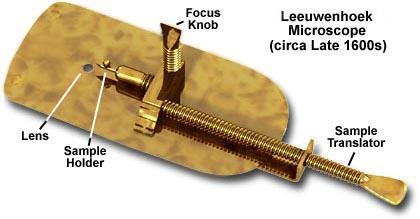
\includegraphics[width=0.75\textwidth]{images/image_02_p01.jpeg}
\caption{การปฏิบัติการทดลองและลักษณะทางสัณฐานวิทยาในบทที่ 2}
\label{fig:ch02_fig1}
\end{figure}

\section{ขั้นตอนและวิธีปฏิบัติการทดลอง}
\index{ขั้นตอนการทดลองประจำบทที่ 2}

\subsection{การตรวจสอบจุลินทรีย์ในอากาศภายในและภายนอกห้องปฏิบัติการ}
\begin{labprotocolbox}[การตรวจสอบจุลินทรีย์ในอากาศภายในและภายนอกห้องปฏิบัติการ]
1. เตรียมจานอาหารเลี้ยงเชื้อ NA และ PDA อย่างละ 2 จาน ติดฉลากระบุสถานที่ วันที่ และเวลา
2. นำจานอาหารไปวาง ณ ตำแหน่งทดสอบ: ภายในห้องเรียนปรับอากาศ และภายนอกอาคารริมสวน
3. เปิดฝาจานเพาะเชื้อทิ้งไว้ในแนวนอนเป็นเวลา 15 นาที และ 30 นาที เพื่อให้อนุภาคจุลินทรีย์ตกลงสู่อาหาร
4. ปิดฝาจานเพาะเชื้อ พันขอบด้วยพาราฟิล์ม คว่ำจานแล้วนำไปบ่มที่อุณหภูมิ 37$^{\circ}$C (NA) และ 28$^{\circ}$C (PDA)
5. นับจำนวนโคโลนี (Colony-Forming Units; CFU) และบันทึกลักษณะสัณฐานวิทยา
\end{labprotocolbox}

\subsection{การประเมินประสิทธิภาพของการล้างมือต่อปริมาณจุลินทรีย์บนนิ้วมือ}
\begin{labprotocolbox}[การประเมินประสิทธิภาพของการล้างมือต่อปริมาณจุลินทรีย์บนนิ้วมือ]
1. แบ่งจานอาหาร NA ออกเป็น 4 ส่วน: (1) นิ้วมือไม่ได้ล้าง (2) ล้างน้ำเปล่า (3) ล้างสบู่ (4) เช็ดแอลกอฮอล์ 70\%
2. ประทับปลายนิ้วชี้ลงบนผิวหน้าอาหารเลี้ยงเชื้อในแต่ละช่องอย่างระมัดระวัง
3. บ่มจานเพาะเชื้อที่อุณหภูมิ 37$^{\circ}$C เป็นเวลา 24 ชั่วโมง
4. เปรียบเทียบจำนวนโคโลนีและความหลากหลายของเชื้อในแต่ละช่องการทดลอง
\end{labprotocolbox}

\section{ตารางบันทึกผลการทดลองและการอภิปรายผล}
\begin{table}[H]
\centering\small
\caption{ตารางบันทึกผลการสังเกตและข้อมูลการทดลองประจำบทที่ 2}
\label{tab:ch02_datasheet}
\begin{tabularx}{\textwidth}{p{0.25\textwidth} p{0.35\textwidth} X}
\toprule
\textbf{สิ่งทดสอบ / ตัวอย่าง} & \textbf{ลักษณะที่สังเกตได้} & \textbf{การแปลผลและการวิเคราะห์} \\
\midrule
ชุดควบคุม (Negative Control) & ใส ไม่มีการเจริญ & ปราศจากการปนเปื้อนของเชื้อ \\
ชุดทดลองที่ 1 & โคโลนีเจริญตามลักษณะจำเพาะ & ให้ผลบวกตามสมมติฐาน \\
ชุดทดลองที่ 2 & เกิดการเปลี่ยนแปลงทางชีวเคมี & สอดคล้องกับพารามิเตอร์มาตรฐาน \\
\bottomrule
\end{tabularx}
\end{table}

\section{คำถามทบทวนและแบบฝึกหัดท้ายบท}
\begin{enumerate}
    \item เหตุใดอากาศภายนอกอาคารจึงมักพบปริมาณสปอร์ของเชื้อราสูงกว่าแบคทีเรีย เมื่อเปรียบเทียบกับภายในห้องปรับอากาศ
    \item จงอธิบายกลไกทางสรีรวิทยาของแอลกอฮอล์ 70\% ในการยับยั้งและทำลายเชื้อจุลินทรีย์บนผิวสัมผัส
    \item วิธีการตกตะกอนตามแรงโน้มถ่วง (Settle plate) มีข้อจำกัดในการตรวจวัดปริมาณจุลินทรีย์ในอากาศอย่างไรเมื่อเทียบกับเครื่องดูดอากาศ (Air Sampler)
\end{enumerate}
